\documentclass{exam}
\usepackage{graphicx}
\usepackage[utf8]{inputenc}
\usepackage[bulgarian]{babel}
\usepackage{amsmath,amsfonts,amssymb}
\title{задачки-закачки-1, гр. 2 и 3}
\begin{document}
\maketitle
\begin{questions}

\question
За кои формални езици $L$ итерацията им $L^*$ е краен език?

\question Докажете, че езикът $L$ е регулярен, където:
\begin{parts}
\part $L = \{w \in \{0, 1\}^* \mid w \text{ е запис на число в двоична бройна система (без водещи нули!)}\}$
\part $L = \left\{ w \in \{0, 1, \dots, 9\}^* \mid w \right.$ е запис на число в десетична бройна система, което се дели на 5, но не и на 25\}
\part $L = \left\{ w \in \{0, 1, 2\}^* \mid w \right.$ е запис на число в троична бройна система с дължина, деляща се на 3\}
\part $L = \left\{ w \in \{a\}^* \mid |w| = 3x + 8y \text{ за някои неотрицателни цели } x, y, \text{за които } x + y > 2 \right\}$
\part $L = \left\{ w \in \{a,b,c\}^* \mid w \text{ съдържа точно 3 пъти буквата } a \right\}$
\part $L = \left\{ w \in \{a,b,c\}^* \mid w \right.$ съдържа точно веднъж буквата $a$, точно два пъти буквата $b$ и точно три пъти буквата $c$\}
\end{parts}

\question Напишете регулярен израз за езика:
\begin{parts}
\part $L = \left\{w \in \{a, b, c\}^* \mid w \right.$ има префикс $abc$ и суфикс $ca$\}
\part $L = \left\{w \in \{a, b, c\}^* \mid w \right.$ не съдържа две последователни еднакви букви\}
\part $L = \left\{w \in \{a, b, c\}^* \mid w \right.$ съдържа три последователни еднакви букви\}
\part $L = \left\{w \in \{a, b, c\}^* \mid w \right.$ съдържа точно веднъж думата $bca$\}
\part $L = \left\{w \in \{a, b\}^* \mid \right.$ в $w$ има поне две последователни букви $b$ след всяко срещане на буква $a$\}
\part $L = \left\{w \in \{a, b\}^* \mid w \right.$ съдържа $ab$ и е с четна дължина\}
\part $L = \left\{w \in \{a, b\}^* \mid \right.$ в $w$ има равен брой срещания на $ab$ и $ba$\}
\part $L = \left\{w \in \{a, b\}^* \mid \right.$ в $w$ се срещат думите $ab$ и $ac$ и последното срещане на думата $ab$ е преди първото срещане на думата $ac$\}
\part $L = \left\{w \in \{a, b\}^* \mid w \right.$ съдържа всяка възможна дума с дължина 2 точно по веднъж\}
\end{parts}

\question Напишете пълен регулярен израз (без да има ... в него) на един ред от тетрадката, който разпознава точно 256 думи над азбуката $\{a, b\}$. А 257? A 255?
\question Знаем, че езикът $L_{()}$ от балансирани скоби не е регулярен. Следните езици регулярни ли са:
\begin{parts}
\part $\{w \in L_{()} \mid |w| \leq 8\}$
\part $\{w \in L_{()} \mid w \text{ е с нечетна дължина}\}$
\end{parts}

\question Да се докаже, че обръщането $L^R$ на регулярен език $L$ е регулярен език.

\emph{Доказателство.} За примитивните регулярни езици имаме $\{\}^R = \{\}, \{\epsilon\}^R = \{\epsilon\}, \{a\}^R = \{a\}$ (значи са регулярни). 
Нека $K^R$ е регулярен за произволен регулярен език $K$, имащ регулярен запис с по-малко от $k > 0$ прилагания на регулярните операции. Нека $L$ е регулярен език, 
имащ регулярен запис с точно $k$ прилагания на регулярните операции. Възможни се следните случаи за $L$:
\begin{itemize}
    \item $L = K_1 \cup K_2$, където $K_1$ и $K_2$ са регулярни и от индуктивното предположение, $K_1^R$ и $K_2^R$ също са регулярни. Тогава $L^R = (K_1 \cup K_2)^R = K_1^R \cup K_2^R$ е регулярен, защото е обединение на регулярни езици.
    \item $L = K_1 K_2$, където $K_1$ и $K_2$ са регулярни и от индуктивното предположение, $K_1^R$ и $K_2^R$ също са регулярни. Тогава $L^R = (K_1 K_2)^R = K_2^R K_1^R$ е регулярен, защото е конкатенация на регулярни езици.
    \item $L = K^*$, където $K$ е регулярен и от индуктивното предположение, $K^R$ също е регулярен. Тогава $L^R = (K^*)^R = (K^R)^*$ е регулярен, защото е итерация на регулярен език.
\end{itemize}
Във всички възможни случаи за $L$ доказахме, че $L^R$ е регулярен. От това по индукция следва, че ако $L$ е регулярен, то и $L^R$ е регулярен.

\question Нека $L \subseteq \{0, 1\}^*$ е регулярен език. Докажете, че следният език е регулярен:
$L' = \{s(w), w \in L \mid s(w) = \text{разменяме нулите и единиците в } w\}$
\question Нека $L$ е регулярен език. Докажете, че ако удвоим всяка буква във всяка дума на $L$, новият език също е регулярен.
\question Нека $L$ е регулярен език. Докажете, че езиците $L_{even}$, съставен от думите на $L$ с четна дължина и $L_{odd}$, съставен от думите на $L$ с нечетна дължина, са регулярни.
\question Нека $A$ и $B$ са регулярни езици над една и съща азбука $\Sigma$. Перфектно картоподреждане $A \clubsuit B$ на $A$ и $B$ наричаме следния език:
\[A \clubsuit B = \{ a_1 b_1 a_2 b_2 \dots a_k b_k \mid a_1 a_2 \dots a_k \in A, b_1 b_2 \dots b_k \in B, a_i \in \Sigma, b_i \in \Sigma\}\]
Да се докаже, че перфектното карторазбъркване на два регулярни езика е регулярен език.
\question Нека $L$ е регулярен език над азбуката $\Sigma$. Да се докаже, че перфектните картораздавания на $L$ са регулярни:
\[L_A = \{a_1 a_2 \dots a_k \mid a_1 b_1 \dots a_k b_k \in L, a_i \in \Sigma, b_i \in \Sigma\}\]
\[L_B = \{b_1 b_2 \dots b_k \mid a_1 b_1 \dots a_k b_k \in L, a_i \in \Sigma, b_i \in \Sigma\}\]

\question Нека $L$ е регулярен език. Да се докаже, че префиксите на всички думи в $L$ образуват регулярен език.
\question Съставете крайни детерминирани автомати за езиците от задачи 2 и 3.
\end{questions}
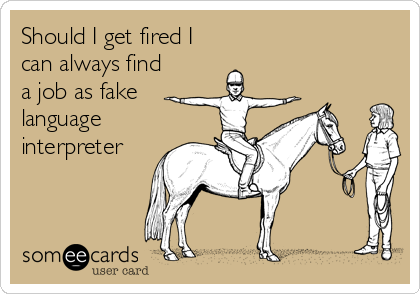
\includegraphics[scale=0.5]{eai}
\end{document}
